\subsection{Models}
To implement an API for the WordCount database, we needed models for the objects we would be sending and receiving from the other layers. 
We also required models corresponding to the database tables to access it through EF Core. The models we have created for communication with other layers and for data access will be described in the following sections.

\subsubsection*{Communication models}
For communication between our layer and the other layers, we have made three input models and one response model. 
These models correspond to the JSON objects we expect to send or receive from other layers when they attempt to insert data into or retrieve data from the database. 
When a JSON object is received, it is parsed into an object from our model, which can then be used to add data to the database.
\\

\textbf{Input models}\\
% ArticleJsonModel
% TermJsonModel
The first input model is \texttt{ArticleJsonModel} which can be seen in figure \ref{ArticlJsonModel}. An article consists of a title, a publisher, a file path, the number of words in the article and an array containing all the words in the article. 
The words are of type \texttt{TermJsonModel} which is a separate model containing the word itself and a number denoting how many times it occurs in the given article.
This model is used when the database receives a JSON object through our endpoint, which corresponds to the \texttt{ArticleJsonModel}. 
After the JSON object has been converted to \texttt{ArticleJsonModel}, the data from the article can be inserted into the WordCount database using EF Core.

\begin{figure}[H]
    \centering
    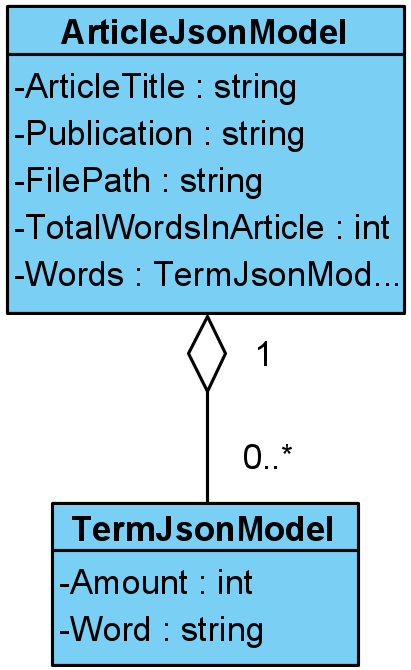
\includegraphics[scale=0.5]{Images/jsonArticleModel.PNG}
    \caption{Diagram of the \texttt{ArticlJsonModel} and the \texttt{TermJsonModel}.}
    \label{ArticlJsonModel}
\end{figure}

% JsonSchemaInputModel
The second input model is \texttt{JsonSchemaInputModel} which can be seen in figure \ref*{JsonSchemaInputModel}. \texttt{JsonSchemaInputModel} contains a name of the JSON schema, and a body which is the JSON schema itself. 
It is used when the other layers try to add JSON schemas to the WordCount database, which is then later used to validate future input. 
How the validation is done will be described in section \ref*{}. \todo{insert ref to validation section}.

\begin{figure}[H]
    \centering
    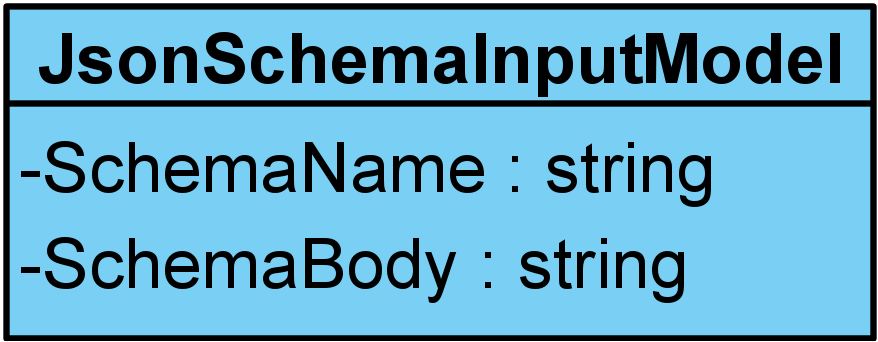
\includegraphics[scale=0.25]{Images/JsonSchemaInputModel.png}
    \caption{Diagram of the \texttt{JsonSchemaInputModel}.}
    \label{JsonSchemaInputModel}
\end{figure}

\textbf{Response Models}\\
% FileIdResponse
The response model \texttt{FileIdResponse} which can be seen in figure \ref*{FileIdResponse}is used when a request for the location of an article is made. 
After the location has been queried on the \texttt{WordCount} database, it is put into the response model, which is returned as a JSON object.

\begin{figure}[H]
    \centering
    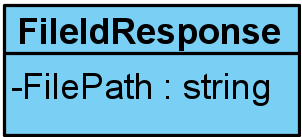
\includegraphics[scale=0.25]{Images/FileIdResponse.png}
    \caption{Diagram of the \texttt{FileIdResponse} model}
    \label{FileIdResponse}
\end{figure}

\subsubsection*{Data access models}
To use EF Core for data access, we also had to implement models of the tables in the database, which can then be used to insert and query data on the database. 
All of these models must be identical to what is on the database, and they are all used the same way by EF Core to manipulate data.
\\
% Article
% publisher
% Term
The model of the \texttt{Article} table along with a \texttt{Term} and a \texttt{Publisher} can be seen in figure \ref*{Article}. 
\begin{figure}[H]
    \centering
    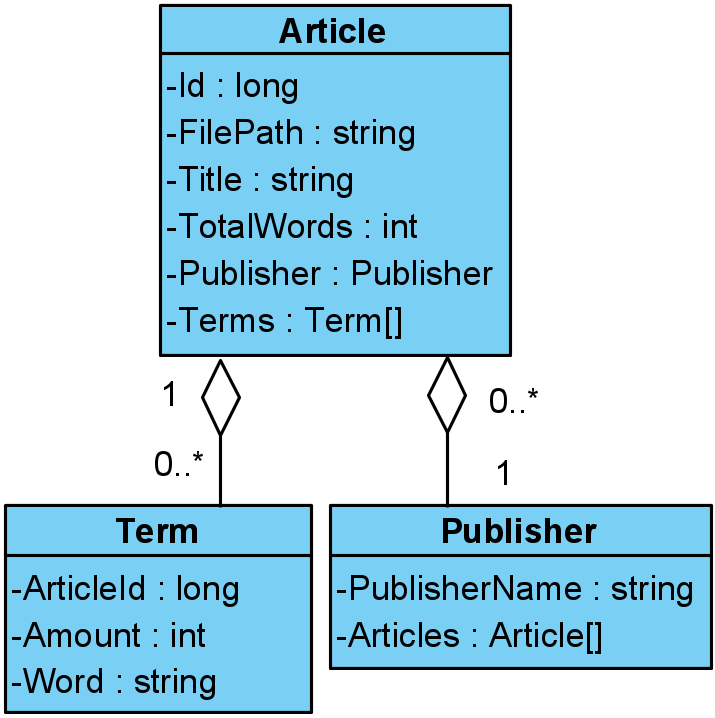
\includegraphics[scale=0.25]{Images/ArticleModel.PNG}
    \caption{Article}
    \label{Article}
\end{figure}
The other models used for database access have  similarly been created to replicate the structure of the database. 
The other models can be seen in appendix \ref*{AppDataAccess}.